\section{Resource Sharing}
Resource sharing, in our context, refers to the ability of microfrontends to efficiently utilize and share common assets, dependencies, and services to minimize redundancy and improve performance. This is one of the areas where our implementation is most lacking.

Although each microfrontend and the Application Shell use the same version of most dependencies, each one still includes its own copy of them. This is a trade-off we have accepted in exchange for the strong isolation provided by Web Components. Using the \texttt{source-map-explorer} package \cite{SourceMapExplorer}, we can analyze the space usage of our bundles through source maps.

Figure \ref{fig:user-usage} shows the results of running this analysis on the \texttt{main.js} file of the User Microfrontend, while Figure \ref{fig:task-usage} presents the results for the \texttt{main.js} file of the Task Microfrontend. In both cases, dependencies (i.e., \texttt{node\_modules}) occupy about 70\% of the total bundle size, whereas the actual application code accounts for only about 30\%. Angular core dependencies comprise approximately 35\% to 40\% of the entire file size. Another significant portion is taken up by the \texttt{chart.js} library, which contributes around 20\% and is used in the dashboard for graph visualizations. The remaining dependencies are relatively small.
\begin{figure}[h]
    \centerline{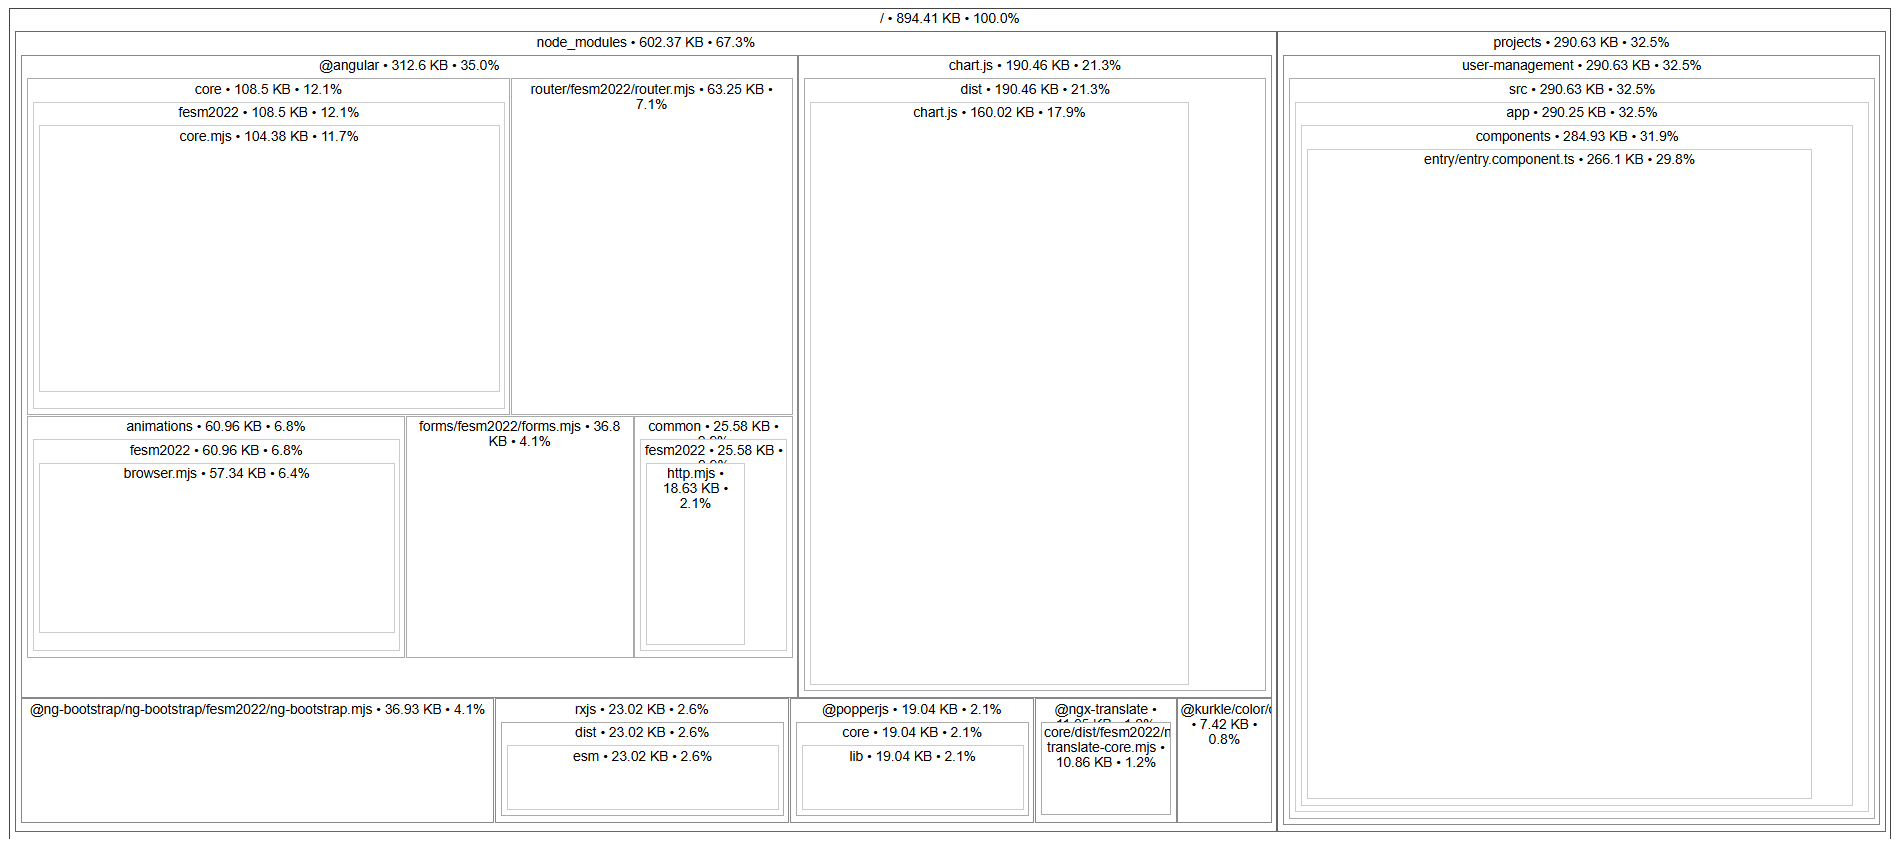
\includegraphics[width=1\textwidth]{images/user-space-usage.png}}
    \caption[Space usage of the User Microfrontend]{Space usage of the \texttt{main.js} file in the User Microfrontend}
    \label{fig:user-usage} 
\end{figure}
\begin{figure}[h]
    \centerline{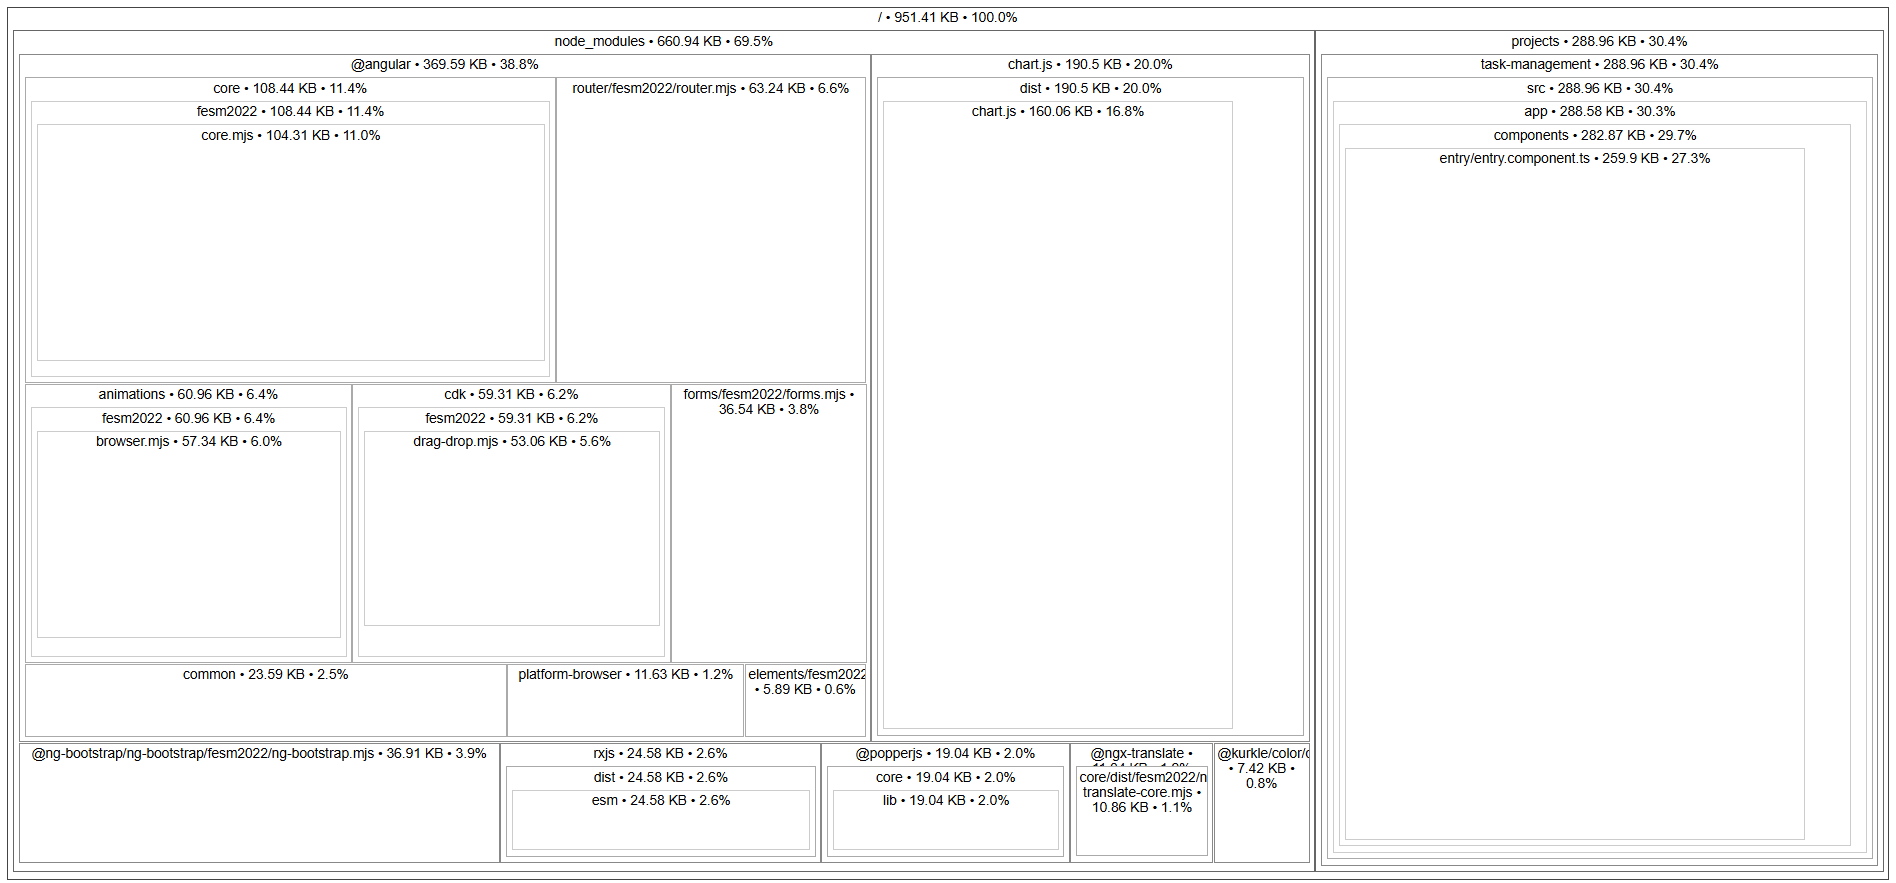
\includegraphics[width=1\textwidth]{images/task-space-usage.png}}
    \caption[Space usage of the Task Microfrontend]{Space usage of the \texttt{main.js} file in the Task Microfrontend}
    \label{fig:task-usage} 
\end{figure}

Based on this analysis, we can conclude that our application would significantly benefit from sharing Angular core dependencies across microfrontends, as well as the \texttt{chart.js} library. However, we were unable to address this issue due to time limitations. One potential solution is to combine the Web Components approach with the Module Federation Webpack plugin—especially since we are already using Webpack.